\documentclass[11pt]{article}
\usepackage{amsmath,amssymb,amsthm}
\usepackage[pdftex]{graphicx}
\usepackage{fancyhdr}
\pagestyle{fancy}

\setlength{\headheight}{0.75in}
\setlength{\oddsidemargin}{0in}
\setlength{\evensidemargin}{0in}
\setlength{\voffset}{-1.0in}
\setlength{\headsep}{10pt}
\setlength{\textwidth}{6.5in}
\setlength{\headwidth}{6.5in}
\setlength{\textheight}{8.5in}

\lhead{}
\chead{Mushroom Classification Project Report}
\rhead{Jim Tao}
\lfoot{}
\cfoot{}
\rfoot{\thepage}
\renewcommand{\headrulewidth}{0.5pt}
\renewcommand{\footrulewidth}{0.3pt}
\setlength{\textwidth}{6.5in}

\begin{document}
\begin{flushleft}
{\em What characteristics make a mushroom most likely to be edible?
What characteristics make a mushroom most likely to be poisonous?
To what extent can we train machine learning models to predict whether a
mushroom is edible or poisonous?}
\end{flushleft}

Data wrangling shows us that the target feature to predict is class
(edible or poisonous), and exploratory data analysis shows us that there
are various pairs of categorical features that are highly correlated
or anti-correlated. After one-hot encoding these categorical features, we
apply and compare five machine learning techniques.
We find that support vector classification (SVC) is 100\% accurate and has the
best explanatory power, although logistic regression and random forest are also
informative and perform just as well with 100\% accuracy.

We are able to determine the four traits most strongly associated with
poisonous mushrooms. They are, in order of importance, green spore prints
(\texttt{r}), creosote odors (\texttt{c}), narrow gills (\texttt{n}), and
silky stalk surfaces above the ring (\texttt{k}), with SVC coefficients
$1.59$, $1.05$, $0.80$, and $0.78$ respectively.
This agrees with the histograms in our exploratory data analysis:
\begin{center}
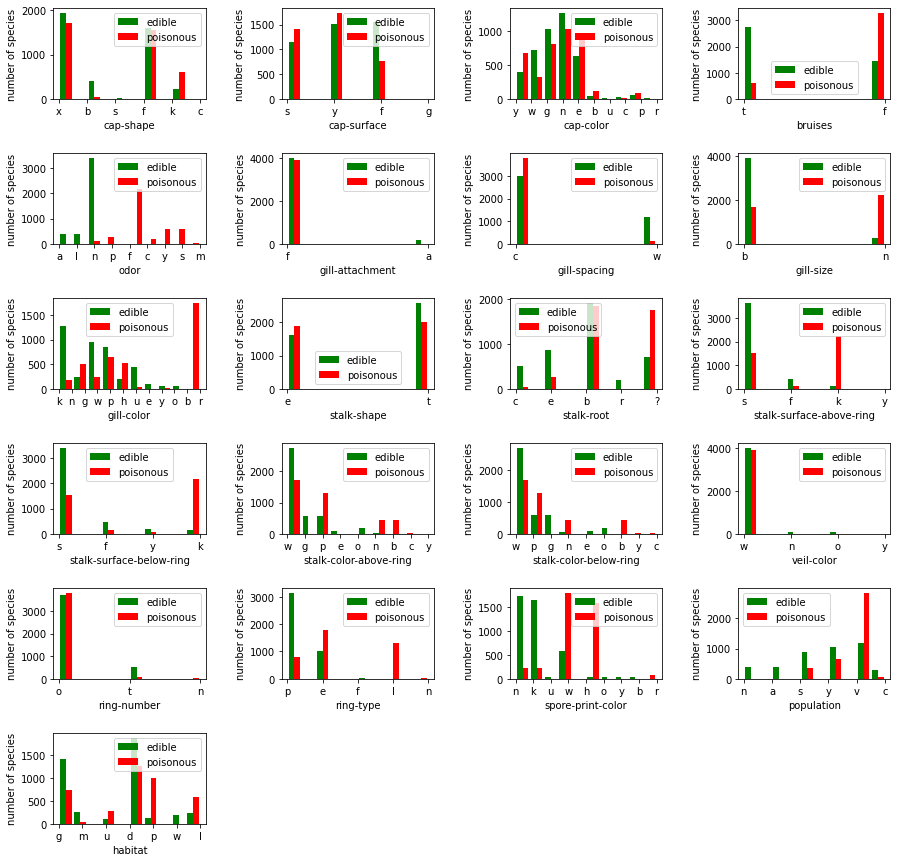
\includegraphics[scale=0.8,trim=460 150 220 570,clip=true]{histograms.png}
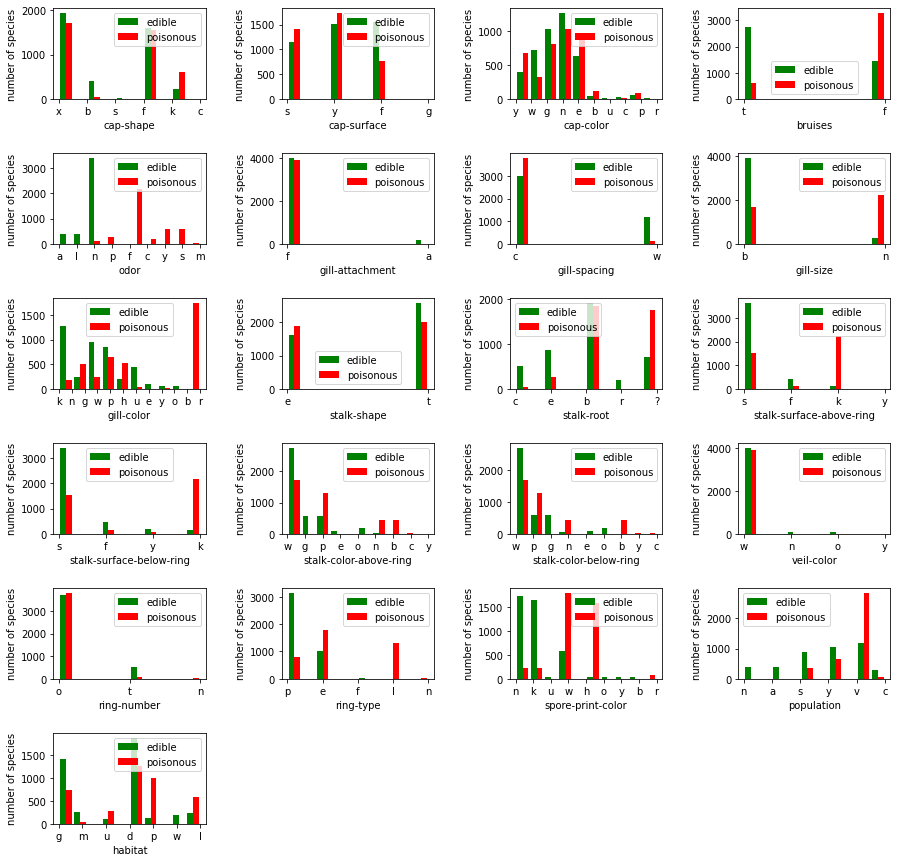
\includegraphics[scale=0.8,trim=0 585 680 135,clip=true]{histograms.png}

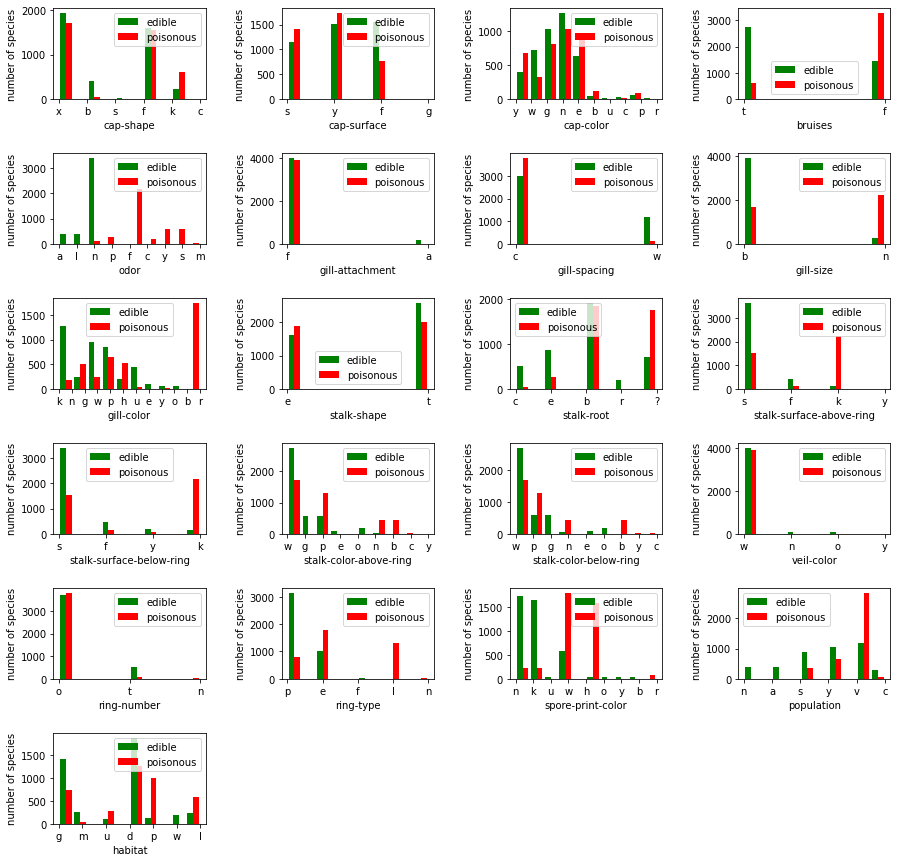
\includegraphics[scale=0.8,trim=680 575 0 145,clip=true]{histograms.png}
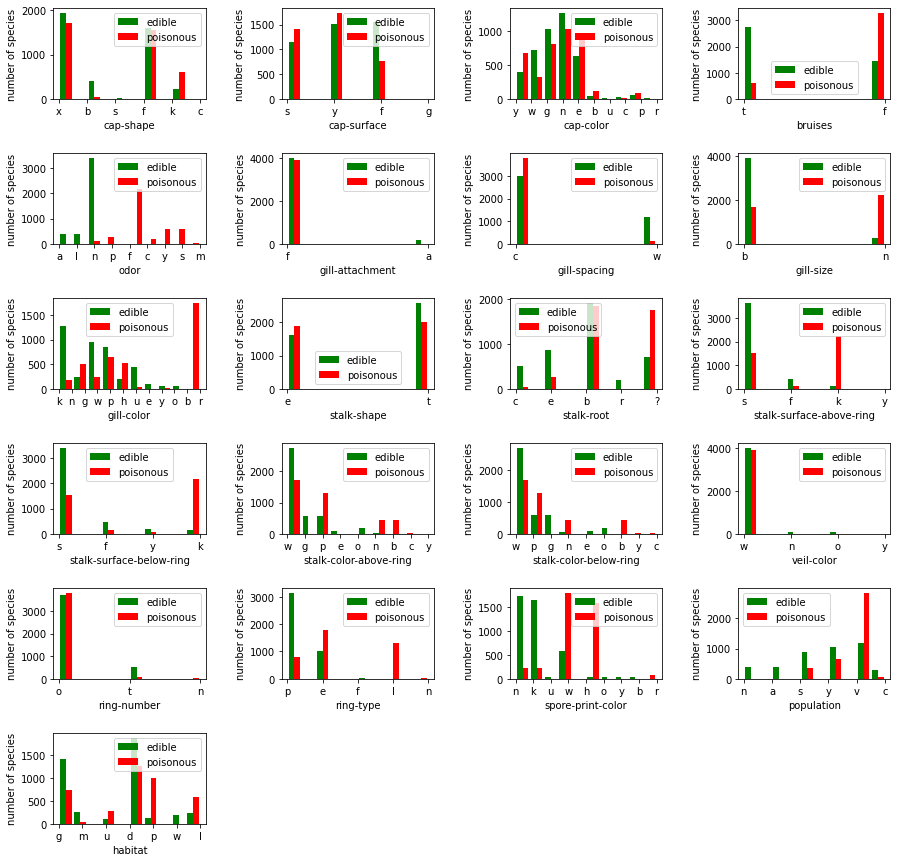
\includegraphics[scale=0.8,trim=680 430 0 280,clip=true]{histograms.png}
\end{center}
We are also able to determine the four traits most strongly
associated with edible mushrooms. They are, in order of importance, almond
odors (\texttt{a}), anise odors (\texttt{l}), no odors (\texttt{n}), and
crowded gill spacing (\texttt{w}), with SVC coefficients 
$-1.02$, $-1.02$, $-0.84$, and $-0.62$ respectively.
This agrees with the histograms in our exploratory data
analysis:
\begin{center}
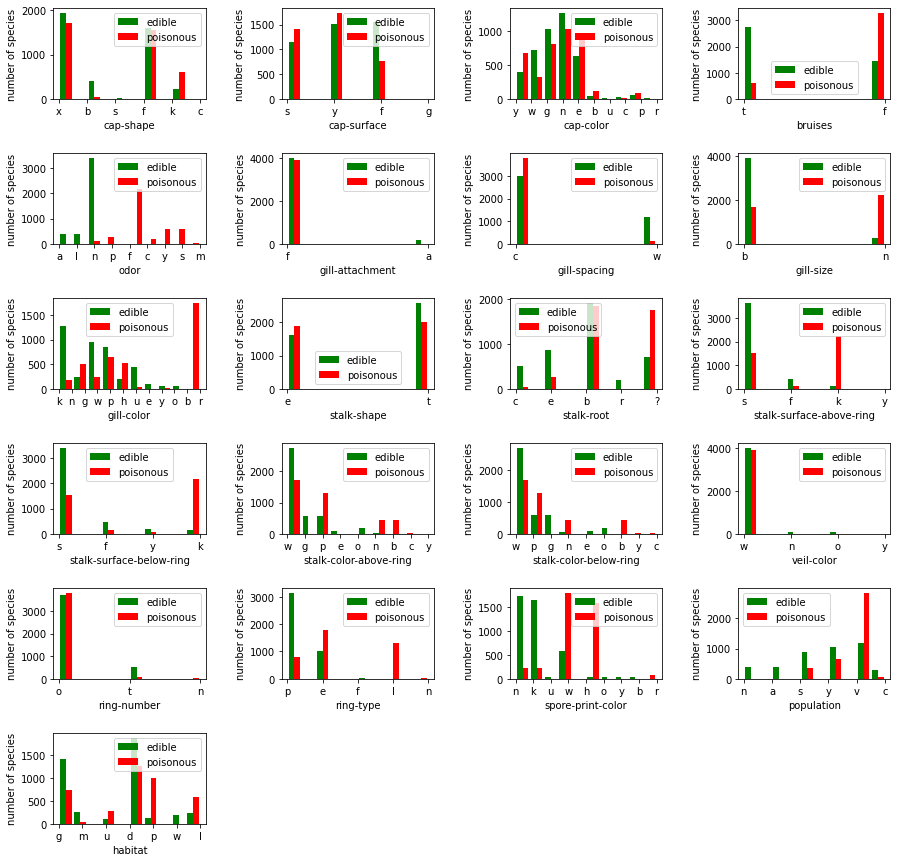
\includegraphics[scale=0.8,trim=0 575 680 145,clip=true]{histograms.png}
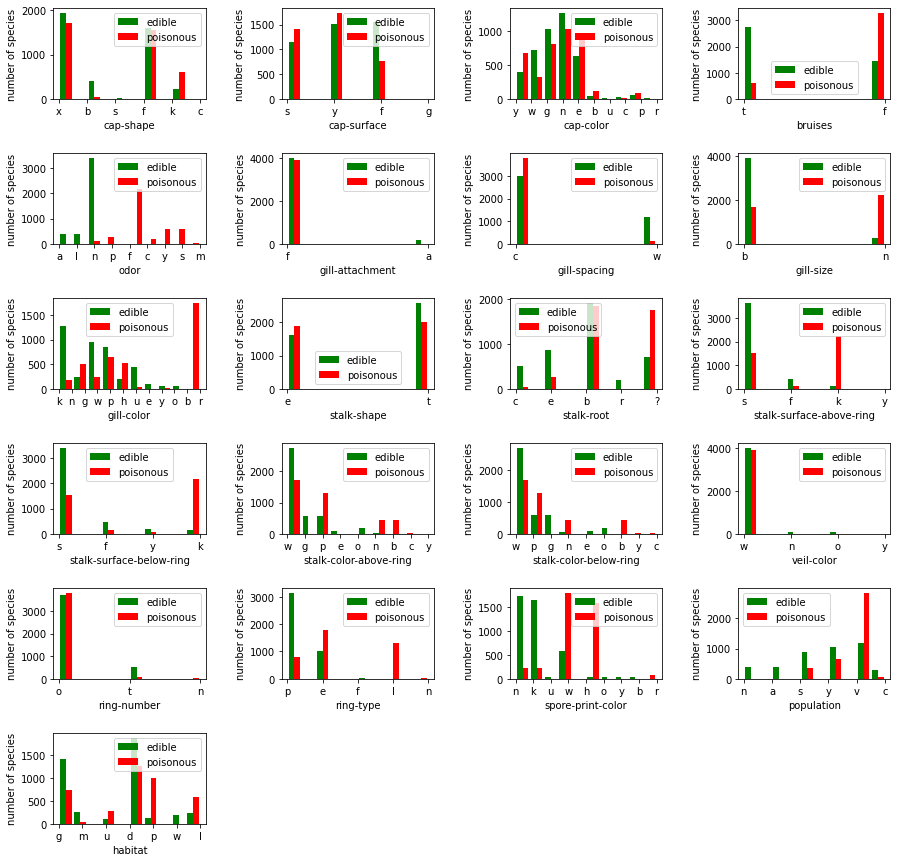
\includegraphics[scale=0.8,trim=460 575 220 145,clip=true]{histograms.png}
\end{center}
\end{document}
